% =============================================================================
% RL setpoint control of a PEM electrolyzer under variable renewable input
% IEEE two-column conference format.
%
% OWNER: Person C (editor-in-chief from Day 4).
%   Person A -> Section III-A, III-B, III-C  (draft prose in notes/A_methodology.md)
%   Person B -> Section III-D, IV            (RL formulation, algorithms, setup)
%   Person C -> everything else
%
% Sections marked \TODO are waiting on Gate G3 (experiment freeze, end of Day 4).
% Nothing else should still be open.
%
% Build:  pdflatex main && bibtex main && pdflatex main && pdflatex main
% =============================================================================
\documentclass[conference]{IEEEtran}
\IEEEoverridecommandlockouts

\usepackage{cite}
\usepackage{amsmath,amssymb}
\usepackage{graphicx}
\usepackage{booktabs}
\usepackage{siunitx}
\usepackage[hidelinks]{hyperref}
\usepackage{xcolor}

\graphicspath{{../results/figures/}}
\newcommand{\TODO}[1]{\textcolor{red}{[\textbf{TODO:} #1]}}
\newcommand{\dVdeg}{\Delta V_{\mathrm{deg}}}

\begin{document}

\title{Reinforcement Learning for Real-Time Setpoint Control of a PEM
Electrolyzer under Variable Renewable Input}

\author{\IEEEauthorblockN{\TODO{authors}}
\IEEEauthorblockA{\TODO{affiliation}}}

\maketitle

% =============================================================================
\begin{abstract}
% Write LAST, after Results. One sentence each: problem, gap, method, result, caveat.
Hydrogen production from proton exchange membrane (PEM) water electrolysis coupled
directly to variable renewable generation is limited less by conversion efficiency than by
stack degradation: the on/off cycling and fast ramping that follow the resource are
precisely the operating patterns that shorten stack life. We formulate real-time
electrolyzer setpoint control as a Markov decision process at a one-minute control
interval and train a reinforcement learning agent to trade hydrogen yield against
cumulative degradation, against a load-following rule-based controller drawn from the
literature. \TODO{one sentence of headline result, from Fig.~\ref{fig:pareto}}
Because the learned policy is characterised as a frontier rather than a single operating
point, the comparison reports the trade-off the controller is actually able to make rather
than a single-axis gain.
\end{abstract}

\begin{IEEEkeywords}
PEM water electrolysis, reinforcement learning, degradation, green hydrogen,
real-time control, variable renewable energy
\end{IEEEkeywords}

% =============================================================================
\section{Introduction}
\TODO{Person C, Day 3.} Cover, in order:
\begin{enumerate}
  \item Green hydrogen and direct renewable coupling; India's National Green Hydrogen
        Mission as a concrete policy hook for the Kutch site.
  \item Degradation is the binding constraint, and intermittency-driven degradation is a
        distinct mechanism from steady-state ageing~\cite{intermittency2025,feng2017pemwe}.
  \item Maximum power tracking is therefore not the right objective.
  \item The gap: prior work hits two of three axes (real-time control / PEM / explicit
        degradation cost). Forward-reference Section~\ref{sec:related}.
  \item Contributions, as a bulleted list.
\end{enumerate}

% =============================================================================
\section{Related Work}\label{sec:related}

\subsection{Degradation in PEM water electrolysis}
Degradation mechanisms in PEM water electrolysis are well catalogued. Feng
\emph{et al.}~\cite{feng2017pemwe} review membrane thinning, catalyst dissolution and
transport-layer passivation, and a recent survey~\cite{bernhardt2026degradation} extends
this across the cell stack together with the diagnostics used to separate the mechanisms.
Microscopic studies of iridium dissolution and redeposition~\cite{yu2020iridium} establish
that the anode is not benign at open circuit, which is why an idle state cannot be treated
as free in any control formulation. Quantitatively, a review of degradation models for
power allocation~\cite{degmodels2025} reports membrane thinning of order
\SI{0.1}{\micro\meter\per\kilo\hour} and catalyst active-area losses approaching
\SI{20}{\percent} over \SI{500}{\hour} under stress conditions.

Most relevant here, a survey of dynamic degradation under renewable
intermittency~\cite{intermittency2025} isolates the mechanisms specific to variable
operation --- on/off cycling, ohmic resistance rise bounded by roughly
\SI{50}{\micro\volt\per\hour}, and thermal fatigue driven by ramping --- and it is these,
rather than steady-state ageing, that a setpoint controller can actually influence.

\subsection{Control of electrolyzers under variable supply}
The simplest and most widely deployed strategy is load following: track the available
resource up to the rated limit and idle below a threshold. We adopt the formulation of
Ref.~\cite{pvt_control_2026} verbatim as our baseline, so that the comparison is against a
published control law rather than one constructed for the purpose.

Degradation-aware control has been addressed with predictive methods.
Ref.~\cite{mpc_refuel_2026} reports that power smoothing under a predictive controller
extends PEM stack life from approximately five to seven and a half years. That work is the
closest non-learning counterpart to ours: it shares the objective but not the method, and
it supplies the lifetime figure against which we calibrate our degradation model
(Section~\ref{sec:calibration}).

\subsection{Reinforcement learning for electrolysis}
Reinforcement learning is now established across power and energy
systems~\cite{cao2020rlreview}. Two studies sit closest to this work, and each differs on
exactly one axis.

Ref.~\cite{awe_rl_2025} trains an RL agent against a physics-informed surrogate to
optimise temperature, flow and current density under renewable input. The method is close
to ours, but the device is a zero-gap \emph{alkaline} electrolyser, whose degradation
physics and dynamic response differ from PEM, and the reward targets efficiency without an
explicit degradation term.

Ref.~\cite{drl_scheduling_2026} applies deep RL to a PEM electrolyzer in an
electric--hydrogen station under a constrained MDP. The device is correct and the method is
RL, but the granularity is \emph{scheduling} --- hour-ahead commitment with discrete
actions --- rather than real-time setpoint control. This distinction is the reason our
control interval is one minute rather than one hour: at hourly resolution the cycling and
ramping mechanisms of Ref.~\cite{intermittency2025} are not resolved at all, and the
control problem reduces to a scheduling problem.

\subsection{Position of this work}
The contribution is the intersection of three properties that prior work satisfies only
two at a time: real-time setpoint control at a sub-hourly interval, a PEM rather than
alkaline device, and an explicit degradation cost inside the reward.
Table~\ref{tab:position} summarises.

\begin{table}[t]
\caption{Position relative to the closest prior work}
\label{tab:position}
\centering
\small
\begin{tabular}{lccc}
\toprule
& Real-time & PEM & Degradation \\
& control & device & in reward \\
\midrule
Surrogate RL, alkaline~\cite{awe_rl_2025}       & \checkmark & --- & --- \\
DRL scheduling, PEM~\cite{drl_scheduling_2026}  & --- & \checkmark & --- \\
Predictive control, PEM~\cite{mpc_refuel_2026}  & \checkmark & \checkmark & --- \\
\textbf{This work}                              & \checkmark & \checkmark & \checkmark \\
\bottomrule
\end{tabular}
\end{table}

% =============================================================================
\section{Methodology}\label{sec:method}

\subsection{Plant model}
\TODO{Person A --- draft prose in \texttt{notes/A\_methodology.md} \S A.}
Summary: Amphlett-form cell voltage with a Nernst pressure correction, Butler--Volmer
activation, ohmic loss and a concentration term; Faradaic efficiency set by hydrogen
crossover. Ohmic resistance and crossover are both derived from a single membrane
thickness, so the two ends of the efficiency curve cannot be tuned independently.
Fig.~\ref{fig:validation} shows the resulting curves.

\begin{figure}[t]
\centering

\includegraphics[width=\columnwidth]{fig_validation.pdf}
\caption{Polarization curve and system LHV efficiency. Efficiency is non-monotonic in
power: crossover dominates at low current density and voltage losses at high current
density, so the setpoint maximising hydrogen \emph{rate} differs from the one maximising
hydrogen \emph{per unit energy}. This is what gives the controller something to decide.}
\label{fig:validation}
\end{figure}

\subsection{Degradation model}
\TODO{Person A --- \texttt{notes/A\_methodology.md} \S B.}
Five terms accumulate into a single scalar cell-voltage rise $\dVdeg$, which feeds back
into the polarization curve so that degradation costs future yield rather than only
reward: a steady-state base rate, a superlinear high-current-density stress term, a
ramp-rate term, a fixed penalty per on/off transition, and an idle term for the anode at
open-circuit potential~\cite{yu2020iridium}.

\subsection{Calibration}\label{sec:calibration}
\TODO{Person A --- \texttt{notes/A\_methodology.md} \S C.}
The five coefficients are not hand-chosen. Each term is linear in its coefficient, so a
single rollout per policy reduces calibration to a small search over coefficient-free
exposure integrals, constrained so that the rule-based baseline of
Ref.~\cite{pvt_control_2026}, driven by the measured resource, reproduces the
approximately five-year stack life reported in Ref.~\cite{mpc_refuel_2026} at an
end-of-life criterion of a \SI{10}{\percent} cell-voltage rise.

\subsection{MDP formulation}
\TODO{Person B.} State, action, reward, episode structure. Reward:
\begin{equation}
r_t = w_1 \, \dot m_{\mathrm{H_2}}(t) \;-\; w_2 \, \Delta V_{\mathrm{deg}}(t)
      \;-\; w_3 \, |\Delta j(t)| ,
\label{eq:reward}
\end{equation}
with $w_2$ swept to trace the frontier of Section~\ref{sec:results}. State the
renewable-only constraint $P_{\mathrm{set}}(t) \le P_{\mathrm{renew}}(t)$ explicitly and
say why: permitting grid backfill collapses the optimal policy onto a fixed
peak-efficiency setpoint and removes the intermittency from the problem.

% =============================================================================
\section{Experimental Setup}\label{sec:setup}

\subsection{Resource data}
The plant is sited at \ang{23.25}\,N, \ang{69.00}\,E in Kutch, Gujarat, India, chosen
because it has strong solar \emph{and} strong wind resource at a single coordinate, so a
solar-heavy versus wind-heavy comparison is not confounded by geography.
\TODO{Confirm provenance before submission --- check
\texttt{data/processed/kutch\_2019\_1min.json}. If the source is \texttt{open\_meteo},
cite ERA5~\cite{hersbach2020era5} and describe the PV~\cite{dobos2014pvwatts} and turbine
conversions as ours; if \texttt{renewables\_ninja}, cite~\cite{pfenninger2016} instead and
state that the conversions are the provider's.}

A full year of hourly data is upsampled to a one-minute interval, since the mechanisms of
Ref.~\cite{intermittency2025} are not resolved at hourly resolution. Sub-hourly structure
is added with an Ornstein--Uhlenbeck cloud-transient process on the solar component and a
turbulence process on the wind component; both are constrained to preserve each hourly
mean exactly, so no energy is introduced by the upsampling. Days are split
\num{293}/\num{72} into training and held-out test sets, stratified by month so that the
test set cannot fall entirely within one season --- a real confound at this site, which has
a pronounced monsoon.

\subsection{Training}
\TODO{Person B.} SAC~\cite{haarnoja2018sac} and PPO~\cite{schulman2017ppo} via
Stable-Baselines3~\cite{raffin2021sb3}; \num{5} seeds; \num{2}M steps; report the device
split and hyperparameters from \texttt{configs/default.yaml}. All reported results are on
held-out days.

% =============================================================================
\section{Results}\label{sec:results}

\subsection{Yield--degradation frontier}
\begin{figure}[t]
\centering

\includegraphics[width=\columnwidth]{fig_pareto.pdf}
\caption{Hydrogen yield against cumulative degradation on held-out days. The learned
policy is shown as a frontier traced by the degradation weight $w_2$ of
Eq.~\eqref{eq:reward}; the two rule-based controllers appear as single operating points.
Error bars are one standard deviation across \num{5} seeds.}
\label{fig:pareto}
\end{figure}
\TODO{Person C, Day 4.} Report the frontier, and state plainly whether the learned policy
dominates each baseline operating point. Do not claim a yield gain that the data does not
support; the frontier is the result.

\subsection{Policy behaviour}
\begin{figure}[t]
\centering
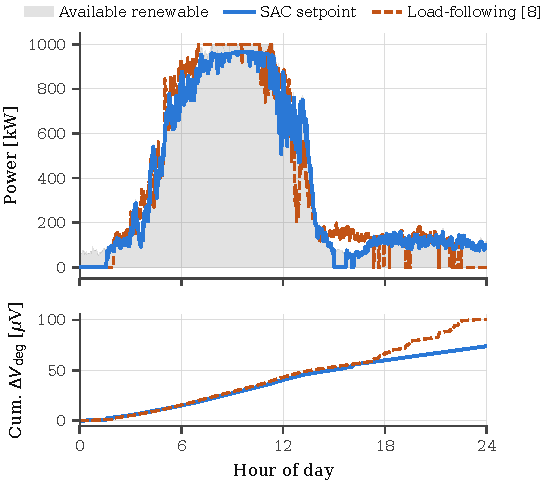
\includegraphics[width=\columnwidth]{fig_trajectory.pdf}
\caption{One held-out day. The rule-based controller follows every transient in the
available resource, while the learned policy declines to, at the cost of some curtailment.
The lower panel shows the resulting difference in accumulated degradation.}
\label{fig:trajectory}
\end{figure}
\TODO{Person C.} This figure explains the frontier rather than asserting it.

\subsection{Sensitivity to the reward weighting}
\begin{figure*}[t]
\centering

\includegraphics[width=\textwidth]{fig_ablation.pdf}
\caption{Effect of the degradation weight $w_2$ on both reward components.}
\label{fig:ablation}
\end{figure*}
\TODO{Person B/C.} Also report solar-heavy versus wind-heavy days, and SAC versus PPO.

\subsection{Long-horizon operation}
\begin{figure}[t]
\centering

\includegraphics[width=\columnwidth]{fig_longhorizon.pdf}
\caption{Cumulative degradation over a \num{90}-day rollout with persistent state, against
the \SI{10}{\percent} end-of-life criterion.}
\label{fig:longhorizon}
\end{figure}
\TODO{Person A/C.} Report projected stack life for each controller.

% =============================================================================
\section{Conclusion and Future Work}
\TODO{Person C, Day 5.}

\subsection*{Limitations}
Three, stated plainly rather than left for a reviewer to find.

First, this is a \emph{simulation study}. No physical stack was operated, and the plant
model, while parameterised from published sources, is not validated against measurement
from the device it represents.

Second, the degradation model is \emph{calibrated from literature-reported rates} rather
than fitted to a measured degradation trajectory. Its absolute scale is anchored to a
single published lifetime figure~\cite{mpc_refuel_2026}; the relative weighting of its
terms follows the mechanisms of Ref.~\cite{intermittency2025} but is not independently
identified. Conclusions about \emph{relative} controller performance are more robust than
any absolute lifetime we report.

Third, we do not compare against model predictive control. MPC is the natural competitor
and has real advantages this work does not claim to displace --- interpretability, and hard
constraint satisfaction by construction. The argument for RL here is narrower: it requires
no explicit dynamics or degradation model at deployment, it can be trained offline on
historical resource data, and it does not re-solve an optimisation at every control step,
which matters at a one-minute interval. A direct comparison is left to future work.

\bibliographystyle{IEEEtran}
\bibliography{refs}

\end{document}
